\chapter{Descri��o Geral}\label{cap:desc}

\section{Perspectiva do Produto}


\section{Fun��es do Produto}

O ambiente deve apoiar a submiss�o e avalia��o autom�tica de
trabalhos pr�ticos, baseados na atividade de teste desenvolvidos
pelos alunos.

\begin{figure}[htbp]
    \begin{center}
        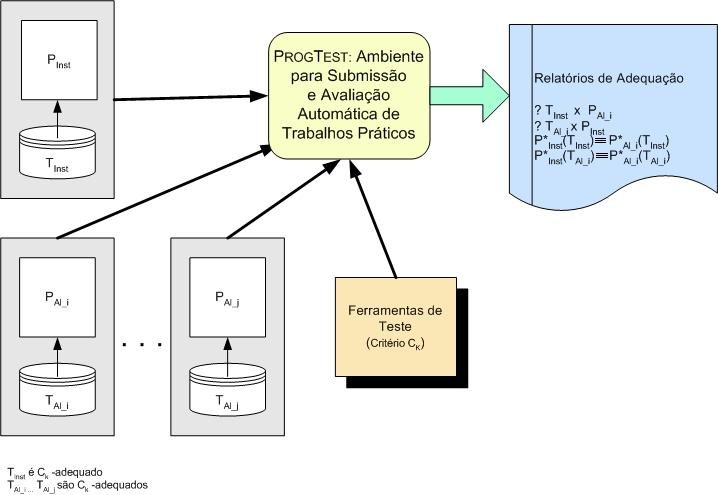
\includegraphics[width=1\textwidth]{figuras/ambiente_novo.jpg}
    \end{center}
    \caption{Ambiente.}
    \label{fig:ambiente_proposto}
\end{figure}

%\section{Caracter�sticas do Usu�rio}
%
%\section{Abrevia��es}
